La QKD (Quantum Key distribution), o Distribuzione Quantistica delle Chiavi, \`e una tecnologia di crittografia quantistica che permette la distribuzione di chiavi crittografiche con un livello di sicurezza inattacabile anche da computer quantistici. La QKD pu\`o essere suddivisa in due macro-classi DV-QKD e CV-QKD. Nella DV-QKD (Descrete Variable Quantum Key Distribution) le informazioni vengono trasmesse utilizzando stati quantici discreti, ad esempio la polarizzazione degli fotoni, che viene misurata attravarso apposite apparecchiature per ogni fotone; al contrario nella CV-QKD (Continous Variable Quantum Key Distribution) vengono misurate variabili continue delle onde elettromagnatiche come ad esempio la fase.

La sicurezza \'e garantita dai principi delle fisica quantistica che ci permettono di rilevare eventuali intercettazioni da parte di una spia (Eve) nella trasmissione su canale quantistico tra Alice (mittente) e Bob (destinatario).

La rilevazione \`e dovuta la fatto che durante la misura da parte de Eve lo stato quantistico viene alterato introducendo del rumore e quindi dell'incertezza. In pratica Eve intercetta lo stato coerente, rappresentato come in figura~\ref{fig:stato-coerente}, ne effettua la misura e lo ritrasmette sul canale. Bob ricever\`a uno stato coerente con del rumore aggiunto, cio\`e la varianza della gaussiana che lo rappresenta \`e maggiore di quella stimata prendendo anche in considerazione in rumore aggiunto dal canale di trasmissione. La detection per\`o, viene effettuata in una fase successiva a quella di trasmissione, durante la quale vengono stimati dei parametri~\ref{subse:stima-parametri} e confrontati con quelli attesi. Nel caso in cui il confronto non vada a buon fine, i parametri stimati e quello attesi differiscono pi\`u di un certo limite stabilito a priori, la trasmissione corrente viene abbortita perch\'e non \`e possibile garantire la sicurezza della chiave crittografica.

\section{CV-QKD con modulazione gaussiana}
Il protocollo di distribuzione quantistica di chiavi a variabili continue con modulazione gaussiana \`e un protocollo molto indicato per lo sviluppo e l'utilizzo su larga scala nel mondo reale data la sua affinit\`a con le infrastrutture oggi gi\`a esistenti, come ad esempio, i canali di comunicazione in fibra ottica. Come enunciato all'inizio del capitolo questo con questo protocollo si effettuano misure su variabili continue delle onde elettromagnetiche e in particolare nei protocolli con modulazione gaussiana gli stati coerenti da trasmettere sul canale di comunicazione vengono estratti da una distribuzione normale centrata in zero e una certa deviazione standard che viene definita in base ad alcuni fattori.

Il protocollo \`e pu\`o essere suddiviso un due sezioni: la prima parte ha effettivamente a che fare con segnali quantistici mentre la seconda parte opera con segnali e dati classici. La prima sezione comprende la scelta e la trasmissione degli stati coerenti su fibra ottica da parte di Alice e termina nel momento in cui Bob effettua la misura; la seconda parte comprende il sifting, la stima dei parametri e la riconciliazione.

\subsection{Trasmissione e misura}
Alice prepara gli stati coerenti andando a estrarre da una distribuzioni normale centrata in zero i valori dell componenti di quadratura \textit{q} e \textit{p}. Dopo la preparazione Alice trasmette a Bob gli stati coerenti attraverso un canale quantistico.

Il canale \`e caratterizzato da un certo valore di trasmittanza e di rumore. A causa della trasmittanza durante la trasmissione il segnale perde potenza quindi le gaussiane che descrivono lo stato coerente saranno centrata in un valore pi\`u vicino allo zero rispetto al momento della preparazione, mentre il rumore che viene introdotto fa aumentare la variaza delle gaussiane cos\`i da accrescere l'incertezza nelle misure da parte di Bob.

Per la misura dello stato coerente possono essere adottati due metodi diversi:
\begin{itemize}
\item \textbf{misura omodina}: Bob decide se misurare la componente di quadratura \textit{q} o \textit{p}, la decisione viene presa con distribuzione di probabilit\`a uniforme.
\item \textbf{misura eterodina}: vengono misurare contemporaneamente entrambe le componenti.
\end{itemize}  

In caso di misura omodina \`e necessaria un'operazione addizionale cio\'e il sifting. Questa operazione consiste nel riverare ad Alice, su canale classico publico, per ogni round quale componente \`e stata misurata da Bob; Alice prende nota delle componenti misurare e scarta le altre.

\subsection{Stima dei parametri}\label{subse:stima-parametri}
Dopo avere terminato la fase di trasmissione degli stati, Alice e Bob rivelano una porzione random di dati in modo tale da confrontare ci\`o che \`e stato effetivamente inviato da Alice con le misure di Bob. Da questo confronto sono in grado di stimare l'effettiva trasmittanza e rumore in eccesso del canale di trasmissione e con queste stime possono calcolare l'informazione mutua $I_{AB}$ (informazione mutua tra Alice e Bob) e l'informazione di Eve $\chi$. Nel caso in cui $\chi$ risulti essere maggiore di $I_{AB}$ il protocollo viene abbortito.

\subsection{Riconciliazione delle informazioni}\label{subse:riconciliazione}
Se la stima dei parametri ha avuto successo Alice e Bob effettuano una correzione degli errori dei segnali scambiati. La riconciliazione pu\`o avvenire in due forme: 

\begin{itemize}
\item \textbf{diretta}: i dati di Alice sono i dati primari e Bob corregge i suoi dati di conseguenza.
\item \textbf{inversa}: in questo caso sono i dati di Bob ad essere i dati primari che vengono inviati ad Alice la quali li utilizza per correggere i propri dati.
\end{itemize} 
 
La riconciliazione diretta presenta un problema, non pu\`o essere utilizzata per valori di trasmittanza troppo bassi, questo perch\'e Eve avrebbe pi\'u informazione sui dati di Alice rispetto a Bob e quindi risulter\`a impossibile creare una chiave crittografica sicura. D'altro canto la riconciliazione inversa non presenta questo problema quindi \`e possibile utilizzarla anche con valori bassi per\`o \`e da tenere in considerazione che pi\`u bassa \`e la trasmittanza pi\`u sar\`a distruttivo l'effetto del rumore del canale.

In questa fase utilizzando la riconciliazione inversa viene generata una chiave crittografica sicura, Bob attraverso dei codici di LDPC (low-density-parity-check) produce una stringa di bit con la quale modulare i propri dati scelti per creare la chiave. Trasmette su canale publico senza errori i propri dati ad Alice la quale li decodifica per ottenere la chiave prodotta da Bob.

\section{Perché funziona, rilevazione di un'eventuale spia}
Questo protocollo \`e particolarmente sicuro prerc\'e consentente il rilevamento di un eventuale spia (Eve), questo \`e possibile grazie a principi delle fisica quantistica. Nel protocollo si assume che Eve sia in possesso di un computer quantistico e che abbia accesso completo al canale di comunicazione e comunque \`e in grado di garantire la sicurezza per diversi tipi di attacchi.

Gli attacchi presi in considerazione tipicamente sono tre e differiscono per la loro efficacia:
\begin{itemize}
\item \textbf{attacchi individuali}: Eve effettua operazioni singolarmente su ogni segnale che viene scambiato tra Alice e Bob. 
\item \textbf{attacchi collettivi}: Eve salva nella memoria del suo computer quantistico un certo numero di stati sui quali effettua una misura collettiva. Questo attacco \`e pi\`u potente del precedente perch\`e secondo i pricipi della fisica quantistica effettuare una misura collettiva si pu\`o potenzialmente ricavare pi\`u informazione che dalla misura del singolo stato. 
\item \textbf{attacchi coerenti}: \textbf{Da chiedere al professore.}
\end{itemize} 

Tornando al motivo per cui effettivamente si riesce a rilevare Eve possiamo dire anche questa volta che \`e merito dei principi della fisica quantistica. Questo perch\`e in caso di misura da parte di Eve lo stato coerente trasmesso verr\`a alterato, quello che avviene in pratica \`e una diminuzione dei fotoni del segnale, quindi per come \`e stato definito il numero di fotoni la rappresentazione dello stato sul piano di Gauss si trover\`a pi\`u vicina all'origine. Inoltre durante la misura viene aggiunto del rumore che comporta una aumento della varianze delle gaussiane che descrivono lo stato e quindi una maggiore incertezza nella misura da parte di Bob.

Tutte questa alterazione, in fase di stima dei parametri, produrranno dei valori indesiderati come $\chi > I_{AB}$. Queste incongruenza tra le stime e ci\`o che ci si aspettava portano a pensare che una spia si sia intromessa nella comunicazione. 


Ancora del testo

\begin{figure}[h] 
\begin{center}
\begin{tabular}{c @{\hspace{1em}} c}
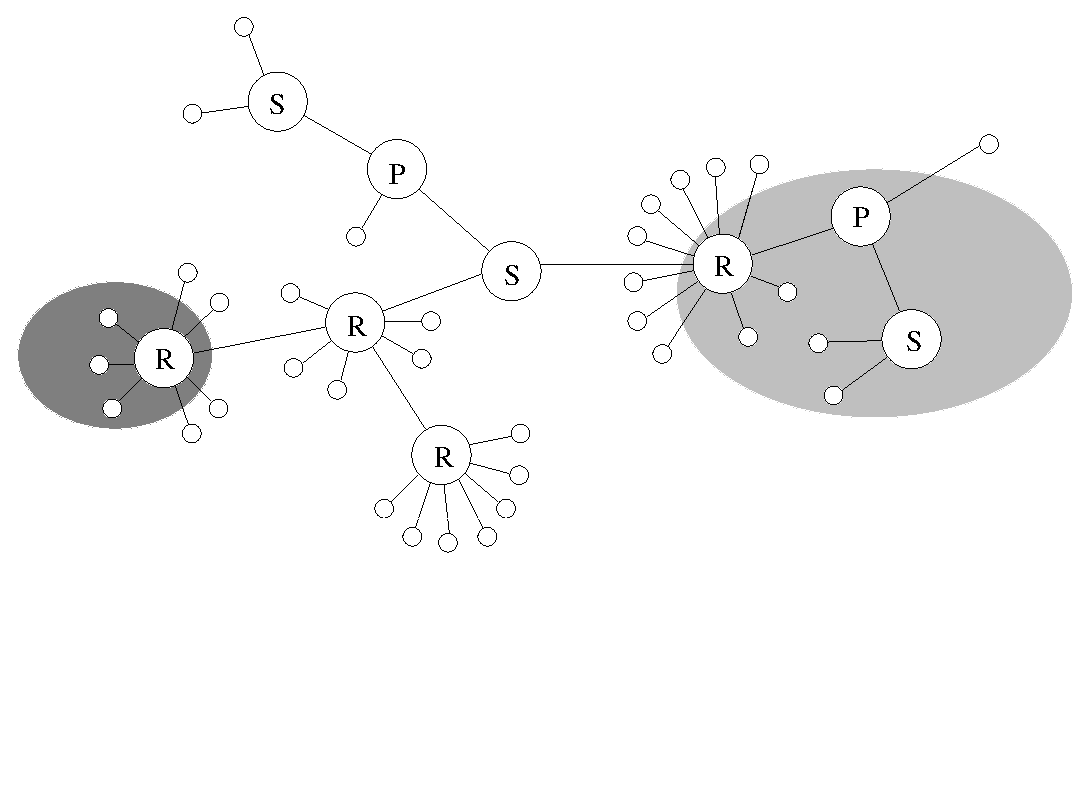
\includegraphics[width=8cm]{figure/esempio-figura-1.eps} &
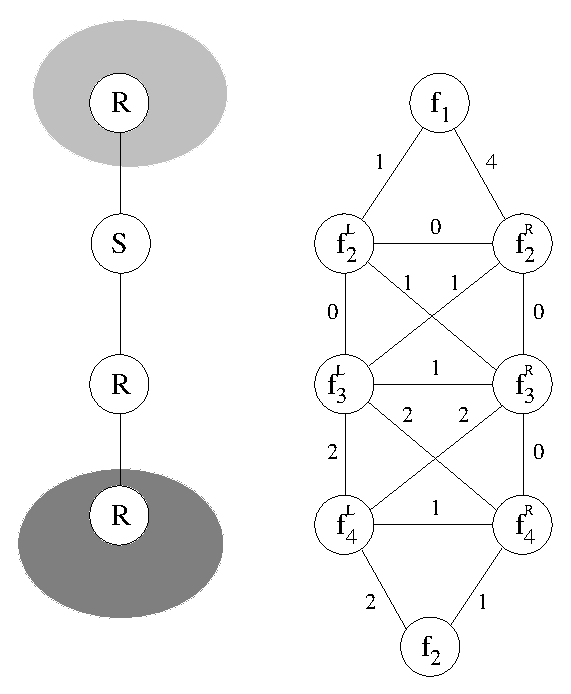
\includegraphics[width=5.5cm]{figure/esempio-figura-2.eps} \\
 (a) & (b)
\end{tabular}
\end{center}
\caption{SPQR-tree di un grafo. (a) L'albero di allocazione della faccia esterna. (b) Il cammino notevole di cui si parla tanto nella Sezione~\ref{se:prima-sezione}.} \label{fig:figura-doppia}
\end{figure}

Come si evince dalle Figure~\ref{fig:figura-doppia}.a e~\ref{fig:figura-doppia}.b non si capisce molto.
